\section{Model Description \label{sec:model}}



The interpretation of the dark matter signal is usually performed with
two approaches: (i) effective field theories (EFTs), and (ii) simplified models. 

\begin{figure}[htbp]
   \centering
   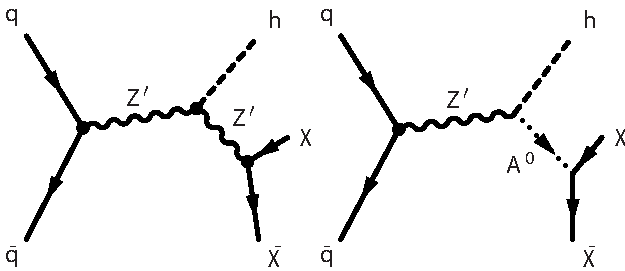
\includegraphics[width=0.7\textwidth]{figures/feyns/feyns.pdf}
   \caption{Left: Feynman diagram of a baryonic Z' model. Right: Feynman diagram of a two Higgs doublet model with a new
     invisibly decaying pseudoscalar \Az from the decay of an on-shell
     resonance \cPZpr\  . Both models give rise to a Higgs+\MET signature. }
   \label{fig:feynman}
\end{figure}

The EFTs assume that DM couples directly to SM particles through a
contact interaction involving a quark-anti quark pair, or two gluons,
and two DM particles and the Higgs particle. The contact interaction 
is described by non-re-normalizable n-dimensional operators. 
Various EFTs operators for the mono-H search are introduced 
and discussed in detail in Ref.~\cite{Irvine}.
%The kinematic distributions are determined by a few parameters: 
%nature and the mass of DM particles, type of operators, 
%and the cut-off scale $\Lambda$. 
The EFTs are valid when the mediators of the interaction between SM and DM 
particles are very heavy; if this is not the case, models that explicitly include 
these mediators are needed (simplified models). 

The ATLAS-CMS DM forum paper~\cite{Abercrombie:2015wmb} recommends three 
benchmark simplified models for the mono-H searches. 
\begin{itemize}
\item  A model where a vector \cPZpr\ is produced resonantly and
  decays into a Higgs boson plus an intermediate heavy pseudoscalar
  particle \Az, in turn decaying into two DM particles, see Fig.~\ref{fig:feynman}.

\item A model where a vector mediator ($\cPZpr_{B}$ ) is exchanged in
  the s-channel, radiates a Higgs boson, and decays into two DM
  particles. In this model, the couplings of the $\cPZpr_{B}$ to
  leptons are omitted.
%
\item A model where a scalar mediator $S$ is emitted from the Higgs
  boson and decays to a pair of DM particles.
%
\end{itemize}

For the time being, we focus on the first two benchmark model. A \cPZpr-two 
Higgs doublet model (\cPZpr-2HDM)~\cite{2HDM} is the first choice to study monoH signal, since the \cPZpr-2HDM is expected to produce, on 
average, a higher \MET value compared to the other two models due to
the on-shell \cPZpr\ production.%, see Fig.~\ref{fig:METmodel}. 


\subsection{ \cPZpr-2HDM model}
In the \cPZpr-2HDM model,
a Type-2 2HDM~\cite{Lee:1973iz,Branco:2011iw} is used to formulate
the Higgs sector, where a doublet $\Phi_u$ couples to up-type quarks, and
a doublet $\Phi_d$ couples to down-type
quarks and leptons. The gauge symmetry of the SM is extended by a
$U(1)_{\cPZpr}$ group, with a new massive \cPZpr\ gauge boson.
Only $\Phi_u$ and right-handed up-type quarks $u_R$ have an associated charge
under the $U(1)_{\cPZpr}$ group, while $\Phi_d$ and all other SM
fermions are neutral.
After electroweak symmetry breaking, the Higgs doublets attain vacuum
expectation values $v_u$ and $v_d$,
resulting in five physical Higgs bosons:
a light neutral CP-even scalar \Ph, assumed to be the
observed 125\GeV Higgs boson, a heavy neutral CP-even scalar \PH,
a neutral CP-odd scalar \Az, and two charged scalars \Hpm.
The analysis in this paper is performed in the context of the so-called
alignment limit where the \Ph\ has SM-like couplings to fermions and gauge
bosons, and the ratio of the vacuum expectation values $\tan \beta = v_u/v_d > 0.3$, as implied from the perturbativity limit of the Yukawa
coupling~\cite{2HDM,Craig:2013hca} of the top quark, the \Ph-\PH mixing angle $\alpha$ is
related to $\beta$ by $\alpha = \beta - \pi/2$.

The benchmark model is parametrized through six quantities: (i) the pseudoscalar mass
\maz, (ii) the DM mass $m_{\chi}$, (iii) the \cPZpr\ mass \mzp,
(iv) $\tan \beta$, (v) the \cPZpr\ coupling strength \gzp, and (vi)
the coupling constant between the \Az and DM particles $g_{\chi}$.

Only the masses \maz and \mzp affect the kinematic
distributions of the objects in the final states studied in this analysis.
In addition, when \Az is on-shell, i.e. $\maz > 2 m_{\chi}$, the kinematics
has little dependence on $m_{\chi}$.
The remaining parameters modify the cross section, branching fraction, and decay
widths of the $\cPZpr$ and the \Az, which leads to only small changes in the
final-state kinematics.



This paper considers \cPZpr\ resonances with mass between 600 and 4000\GeV and 
\Az particles with mass between 300 and 800\GeV. The mass of the DM particles $m_{\chi}$
is assumed to be less than or equal to 100\GeV. The parameters $\tan \beta$ and $g_{\chi}$ are fixed at unity.
Hypotheses for the mass of the \Az particle to be less than 300\GeV are excluded by constraints on flavor changing
neutral currents from measurements of $\cPqb\rightarrow \cPqs\gamma$ \cite{Branco:2011iw},
and therefore are not considered. The branching fraction of the \Az particle to dark matter (${\cal B}(\Az\rightarrow\chi\overline{\chi})$) decreases as $m_{\chi}$ increases.
For the mass range of the \Az particle considered in this paper, the relative drop of
${\cal B}(\Az\rightarrow\chi\overline{\chi})$ when $m_{\chi}$
increases from 0 to 100\GeV is within 7\% . Therefore, the result obtained with the assumption of $m_{\chi}= 100\GeV$ is considered valid also for $m_{\chi}\leq 100\GeV$.
The value of ${\cal B}(\Az\rightarrow\chi\overline{\chi})$ is approximately $100\%$ for \Az particles of $300\GeV$ in mass.
The branching fraction starts to decrease when the mass of the \Az particle is more than twice the mass
of top quark, since the $\Az\rightarrow$ $\cPqt\cPaqt$ decay channel becomes kinematically
accessible. For \Az particles of masses between if 400 and 800 $\GeV$ the branching fraction is reduced to values that range from 54 to 42$\%$. In this paper the branching fraction ${\cal B}(\Az\rightarrow\chi\overline{\chi})$ is forced to be 100 $\%$ for all the considered mass hypotheses.
% and the results are presented in terms of exclusion limits of decays to
%DM particles and the signal cross section includes
%the value of ${\cal B}(\Az\rightarrow\chi\overline{\chi})$.

The quantity \ptvecmiss, calculated as the negative vectorial sum of the transverse momentum (\pt) of all objects identified in an event, 
represents the total
momentum carried by the DM particles.
The magnitude of this vector is referred to as \MET.
For a given value of \mzp, the \pt of the \Az decreases as its mass increases.
Therefore, the \MET spectrum softens with increasing \Az masses.
%A comparison of the \MET distributions for three values of the mass of the \Az particle is shown in Fig.~\ref{fig:mA0}.

%\begin{figure}[htbp]
%\centering
%\includegraphics[width=0.45\textwidth]{figures/Figure_002.pdf}
%\caption{Distribution of \MET at generator level for \cPZpr\ $\rightarrow$ h\Az\ $\rightarrow$ h$\chi\chi$ with \maz = 300, 500, and 700\GeV with \mzp = 1200\GeV. All other parameters of the model are fixed, as mentioned in the text.}
%\label{fig:mA0}
%\end{figure}

The signal cross section times branching fraction is calculated
for the fixed value of \gzp = 0.8, as considered in Ref.~\cite{ATLAS-2015-PAS} and recommended in
Ref.~\cite{Abercrombie:2015wmb}. 


%In the 2HDM model of Ref.~\cite{2HDM}, a Type-2 two Higgs doublet is assumed, where 
%$\Phi_u$ couples to up-type quarks and $\Phi_d$ couples to down-type
%quarks and leptons. The gauge symmetry of the SM is extended by a
%$U(1)_{\cPZpr}$, with a new massive \cPZpr\ gauge boson. In this 2HDM
%model, only $\Phi_u$  and right-handed up-type quarks $u_R$ are charged 
%under the $U(1)_{\cPZpr}$ while $\Phi_d$ and  all the other SM
%fermions are neutral. 
%
%After electroweak symmetry breaking, the Higgs doublets attain vacuum 
%expectation values $v_u$ and $v_d$, and in unitary gauge the doublets are
%parametrized as
%
%\[
%\Phi_d = \frac{1}{\sqrt{2}}
%\begin{pmatrix}
% -\sin\beta~\PH^+\\
%v_d - \sin\alpha~\Ph + cos\alpha~\PH - i \sin\beta~\Az
%\end{pmatrix},
%\]
%
%
%\[
%\Phi_u = \frac{1}{\sqrt{2}}
%\begin{pmatrix}
% \cos\beta~\PH^+\\
%v_u + \cos\alpha~\Ph + sin\alpha~\PH + i \cos\beta~\Az
%\end{pmatrix},
%\]
%
%where \Ph, \PH\ are neutral CP-even scalars, \Hpm\ is a charged scalar,
%and \Az\ is a neutral CP-odd scalar. In this framework,
%$\tan\beta\equiv v_u/v_d$, and $\alpha$ is the mixing angle that diagonalizes
%the $\Ph-\PH$ mass squared matrix. This model also contains an
%additional scalar singlet $\phi$ that leads to spontaneous symmetry
%breaking. The $\alpha$ is assigned to be $\alpha = \beta - \pi/2$, 
%in the limit where the \Ph\ has SM-like couplings to fermions and gauge
%bosons, and $\tan \beta \geq 0.3$ as implied from the perturbativity
%of the top Yukawa coupling. 
%
%The model is described by five parameters:
%\begin{itemize}
%\item the pseudoscalar mass $M_{\Az}$,
%\item the DM mass $M_{\chi}$,
%\item the \cPZpr\ mass $M_{\cPZpr}$,
%\item $\tan \beta$,
%\item the  \cPZpr\ coupling strength $g_z$.
%\end{itemize}
%
%However, only the masses $M_{\Az}$ and $M_{\cPZpr}$ affect the 
%kinematic distributions as shown in Section~\ref{sec:sigSamp}. 
%All the other parameters affect the cross sections and decay widths only.
%
%The decay width of $\cPZpr\rightarrow \Ph
%\Az$ is:
%\begin{equation}
%\Gamma_{\cPZpr\rightarrow\Ph\Az}= \left(g_z
%  \cos\alpha\cos\beta\right)^2 \frac{\left | p\right|}{24\pi}\frac{\left | p\right| ^2}{M_{\cPZpr}^2},
%\end{equation}
%where $|p|$ is the center of mass momentum for the decay products
%
%\[
% |p| = \frac{1}{2M_{\cPZpr}} \sqrt{
%   \left(M_{\cPZpr}^2-\left(m_{\Ph}+m_{\Az}\right)^2\right) 
%\left(M_{\cPZpr}^2-\left(m_{\Ph}-m_{\Az}\right)^2\right)}.
%\]
%
%The cross sections listed in Section~\ref{sec:sigSamp} were computed assuming  $g_Z=0.08$ in Eqn~\ref{eq:gz}.
%
%



\subsection{ \cPZpr-Baryonic model}
A Z' vector boson is a well-motivated feature of many new physics scenarios. 
The Z'-motivated DM models are more interesting since the corresponding U(1)' 
gauge symmetry ensures DM stability. The model is an extension of the SM and 
assumes that the baryon number (B) is gauged, with the Z' being the gauge 
boson of U(1)$_{B}$. The consistency of theory requires the existence of new 
stable baryonic state that are neutral under SM gauge symmetry. This new 
particle is an excellent DM candidate. If the DM particle carries a baryon 
number $B_{\chi}$, the Z'-quark-DM part of the Lagrangian for models with 
fermionic dark matter is 
\begin{equation}
{\cal L} = g_q \bar{q}\gamma^{\mu}q\cPZpr_{\mu}+g_{\chi}\bar{\chi}\gamma^{\mu}\chi\cPZpr_{\mu}
\end{equation}
To generate the Z' mass, a ``baryonic Higgs'' scalar is introduced to 
spontaneously break the U(1)$_B$ symmetry. Analogous to the SM, there remains 
a physical baryonic Higgs particle, $h_{B}$, with a coupling of h$_{B}$Z'Z' 
and vacuum expectation value of v$_{B}$. 
The \cPZpr\ and SM Higgs boson h interact with a coupling strength of 
$g_{h\cPZpr\cPZpr} = m_{\cPZpr}^{2} \sin \theta/v_{B}$, where $\theta$ is the h-h$_{B}$ 
mixing angle. This allows for mono-Higgs final states at the LHC as shown in 
Fig.~\ref{fig:feynman}. In the search for this model, values for $g_q$ and $g_\chi$ are chosen to be 0.25 and 1, respectively. The ratio $g_{h\cPZpr\cPZpr}/M_{\mathrm{Z}'}$ is chosen to be unity. All these parameter choices follow the recommendations from~\cite{Abercrombie:2015wmb}.  



\begin{figure}[htbp]
   \centering
   \includegraphics[width=0.7\textwidth]{figures/models/gq0p3333_ZpBaryonic_MSC500_MDM1_gq0p25_ZpBaryonic_MSC500_MDM1.pdf}
   \caption{Comparison of the generator-level \MET\ distributions predicted 
by the \cPZpr-Baryonic model (after parton shower by \PYTHIA) for $g_q=0.25$ and $g_q=0.3333$. The mass of 
the dark matter particle is set to 1~\GeV and the mass of the mediator 
\cPZpr\ is set to 500~\GeV, respectively. Samples for this model have been generated with $g_q=0.3333$; however, as the kinematics does not change, we use them to interpret the results under the assumption $g_q=0.25$ by appropriately rescaling the cross section.}
   \label{fig:METZpBgq}
\end{figure}

\begin{figure}[htbp]
   \centering
   \includegraphics[width=0.45\textwidth]{figures/models/xsec_ZBToDMSimp.pdf}
   \includegraphics[width=0.45\textwidth]{figures/models/width_ZBToDMSimp.pdf}
   \caption{Ratios of the leading-order mono-jet cross sections (left) 
and $\Gamma_{\cPZpr}$ (right) predicted by the \cPZpr-Baryonic model 
relative to that 
predicted by {\sc DMSimp-spin1}. The ratios are consistent with unity.
}
   \label{fig:ZBXsWidth}
\end{figure}




The \MET distributions for many different mass combinations for both models investigated are shown in Fig.~\ref{fig:puppimet_models}. 

\begin{figure}[htbp]
   \centering
   \includegraphics[width=0.43\textwidth]{figures/models/puppimet_signals_2hdm.pdf}
   \includegraphics[width=0.43\textwidth]{figures/models/puppimet_signals_barzp.pdf}\\
   \includegraphics[width=0.43\textwidth]{figures/models/puppimet_signals_2hdm-300.pdf}
   \includegraphics[width=0.43\textwidth]{figures/models/puppimet_signals_barzp-1000.pdf}\\
   \includegraphics[width=0.43\textwidth]{figures/models/bbdR_signals_2hdm.pdf}
   \includegraphics[width=0.43\textwidth]{figures/models/bbdR_signals_barzp.pdf}\\
   \caption{\ptmiss distributions  for different $M_{\text{Z'}}$ for the Z'-2HDM (upper left) and for the Z'-Baryonic model (upper right); \ptmiss distributions for different $M_{A^0}$ in the Z'-2HDM (middle left) and for different $M_\chi$ (middle right). Lower row: distance between the two b quarks coming from the Higgs boson decay.}
   \label{fig:puppimet_models}
\end{figure}


A direct comparison of the \MET~spectra for the \cPZpr-2HDM and the Baryonic $Z'$ model for similar $M_{\text{Z'}}$ are shown in Fig.~\ref{fig:puppimet_signals}.

\begin{figure}
   \centering
   \includegraphics[width=0.6\textwidth]{figures/puppimet_signals.pdf}
   \caption{\ETslash~spectra for the signal models investigated. The Baryonic $Z'$ model has a significantly softer spectrum.}
   \label{fig:puppimet_signals}
\end{figure}
